
\section{Trees}
\label{sec:trees}

When we use a list for storing our data in a dynamic structure, 
there are two limitations: 

\begin{itemize}
\item Finding an element in the list takes a long time, proportional
  to the length of the list.
\item Keeping  the list's elements sorted also takes a lot of
  time: you must find the place where the new element should be, and
  then insert it. 
\end{itemize}

Both seeking an element and inserting an element in a list require a
time that is proportional to the length of the list. They will take
(in average) twice as long in a list twice as big. 

We have seen that \emph{maps} provide a partial solution to the first
problem. By assigning a value with a key, they can access any element
immediately. However, maps have some problems too. Either you store
the keys on an array that you can access by index (i.e.~a hash of the
key) ---which is not dynamic---
or you need a linked list of keys ---which has similar problems: it
may require a lot of time to find a key---. 

Generally speaking, maps are used for relatively low numbers of
elements. When the number of elements is very big, and it 
is important to have them sorted, there is a better data structure:
the tree. 

A tree in computing is similar to a tree in nature because it has a
root and it has branches. Like a linked list, a tree is composed of
elements. Elements where branches start are usually called
\emph{nodes} and elements at the end of branches are usually
\emph{leaves}. In some trees you have data on nodes and leaves, while
in others you have data only on leaves. 

Trees are very important in computing. For example, the filesystem on
your hard disk, where you have stored all your files (including this
file you are reading now, your personal folders/directories, etc) has
a tree structure: folders are nodes and files are leaves. 

Trees have a similar structure to lists, stacks, and queues; the main
difference is that each element points to two or more elements instead
of one. See this example: 

\begin{figure}[hbtp]
  \centering
  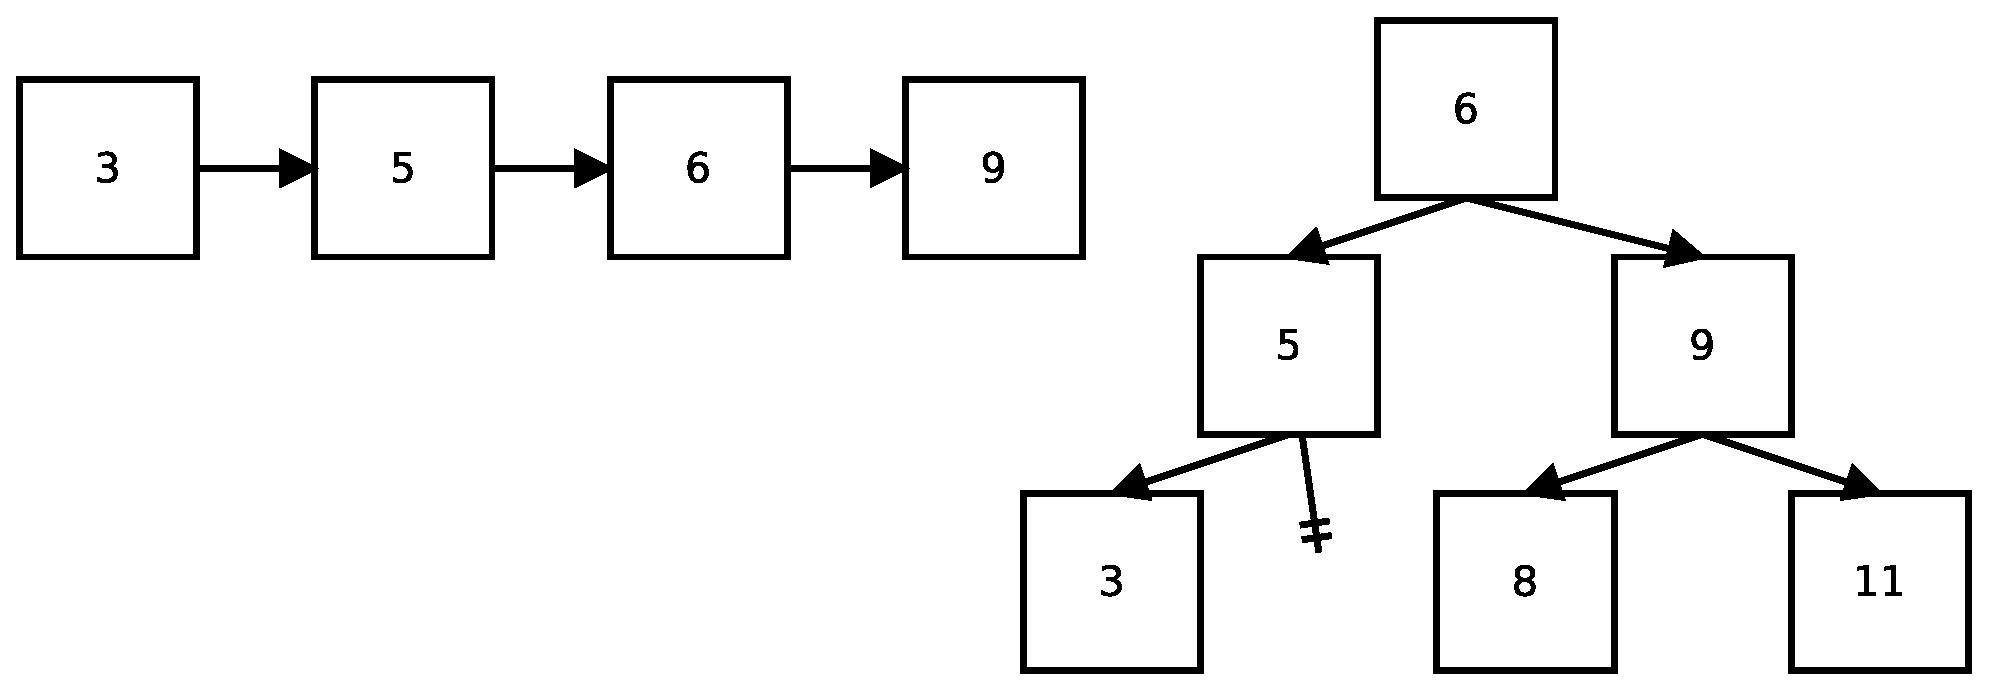
\includegraphics[width=\textwidth]{gfx/list-tree}
  \caption{In a singly-linked list, every element is connected to the
    next one. In a binary tree, every element is connected to two next
    elements. It is usual to draw trees going down (like when we
    write in English) rather than going up (as trees in Nature).}
  \label{fig:listree}
\end{figure}

\begin{verbatim}
    public class IntegerListNode {
        int value;
        IntegerListNode next;
        // ... methods would be here
    }
    (...)
    public class IntegerTreeNode {
        int value;
        IntegerTreeNode left;
        IntegerTreeNode right;
        // ... methods would be here
    }
\end{verbatim}

Trees where every node links to two other nodes are called
\emph{binary trees}. Binary trees are the most common types of
trees, but we can create trees of any cardinality (see the examples
below). Although we are going to focus on binary
trees in this section, everything we will learn can be applied to
any type of tree. 

{\small  % If not small, does not fit
  \begin{verbatim}
  public class IntTernaryTreeNode {   public class IntArbitraryTreeNode {
     int value;                             int value;
     IntegerTernaryTreeNode left;           IntArbitraryTreeNode[] children;
     IntegerTernaryTreeNode center;         // ... methods would be here
     IntegerTernaryTreeNode right;    }
     // ... methods would be here
  }
  \end{verbatim}
}

\subsection{Adding elements to a tree}
\label{sec:adding-elements-tree}

Trees have a structure that makes it very easy to keep the data
sorted. This is important because it is faster to find a specific
piece of data when everything in order.. 

When we want to add a new element to a tree we start at the root. Then
we check whether we want to add it to the right or to the left. Then
we continue the process on that branch. Let's see an example based on 
clas \verb+IntegerTreeNode+ above.

\begin{verbatim}
    public add(int newNumber) {
        if (newNumber > this.value) {
            if (right == null) {
                right = new IntegerTreeNode(newNumber);
            } else {
                right.add(newNumber);
            }
        } else {
            if (left == null) {
                left = new IntegerTreeNode(newNumber);
            } else {
                left.add(newNumber);
            }
        }            
    }
\end{verbatim}

You can see that the process is symmetrical: we decide to go left or
right based on the new number to add, and then we continue on that
side of the tree. This leaves the three automatically sorted: ``lowers''
on the left, ``highers'' on the right, at every level of the tree. If
there is nothing in the branch, we add our new element; otherwise, we
compare again. 
Note that the first element of the tree (i.e.~the
root) may need to be handled as a special case (as with
lists). Figure~\ref{fig:treecr} shows how a tree is created by adding
some new nodes. 

\begin{figure}[hbtp]
  \centering
  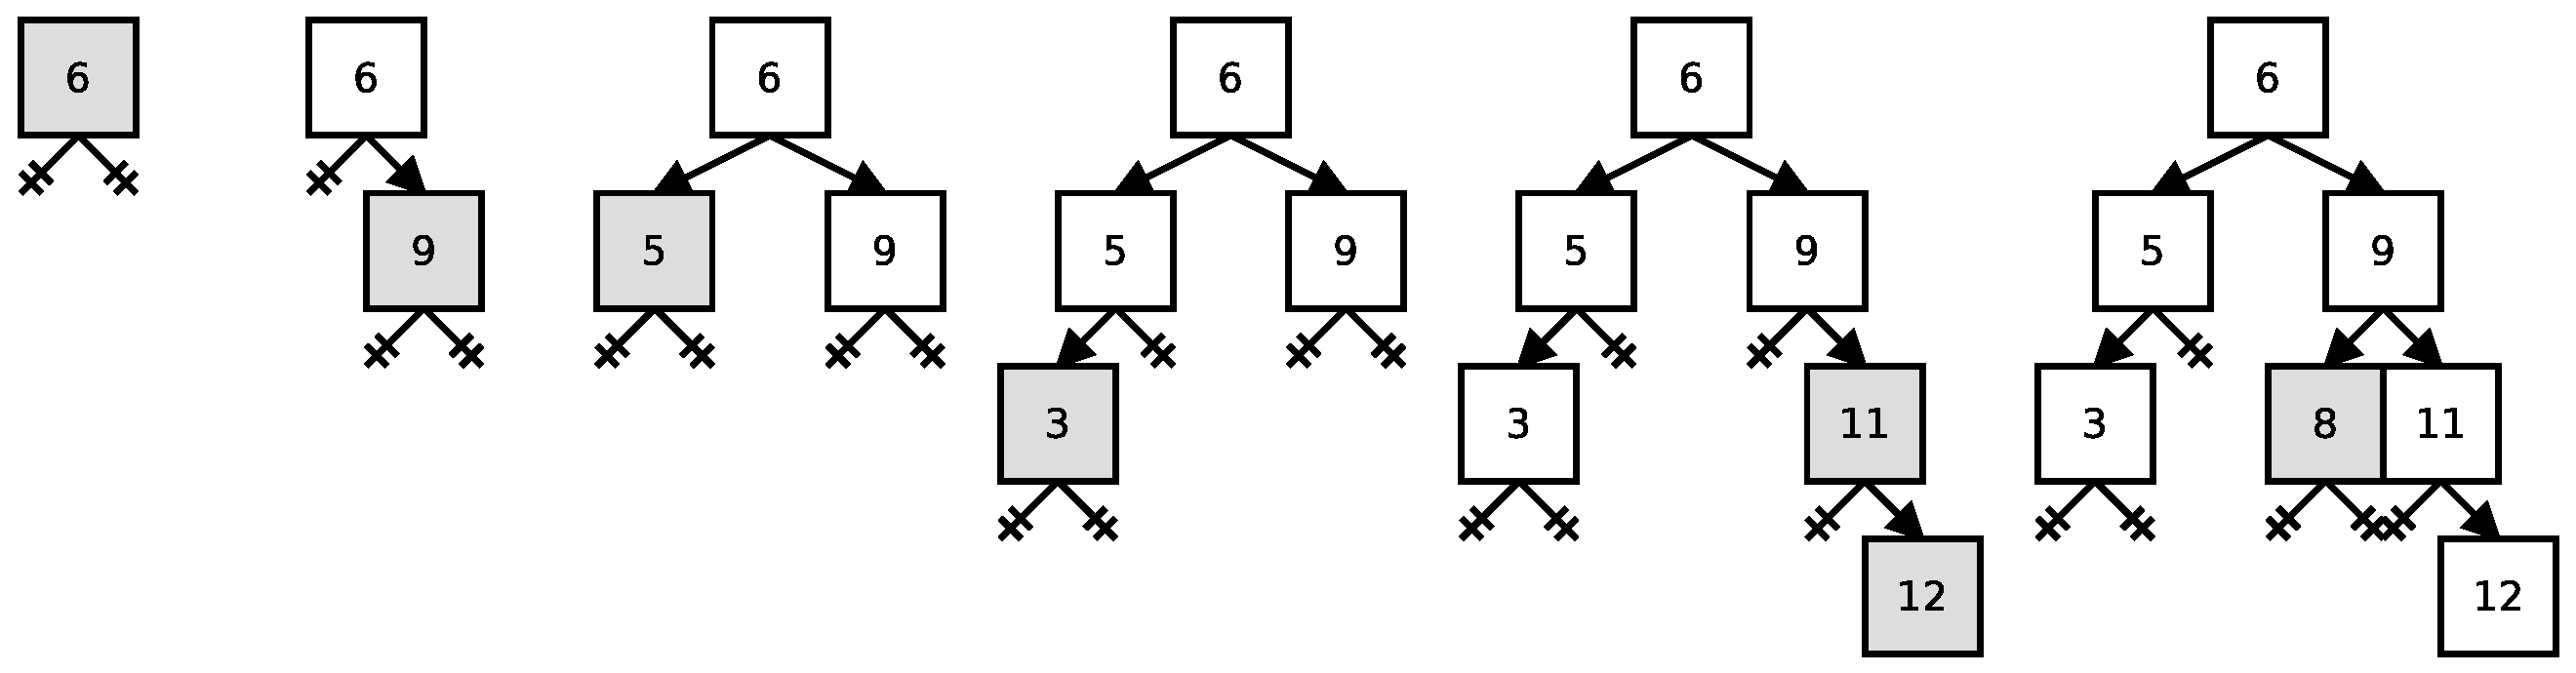
\includegraphics[width=\textwidth]{gfx/tree-creation}
  \caption{Creation of a tree based on the class IntegerTreeNode and
    its method add(int). The numbers are added unsorted as 6, 9, 5, 3,
    11, 12, 8\ldots} 
  \label{fig:treecr}
\end{figure}

\subsection{Finding elements in a tree}
\label{sec:find-elem-tree}

The good thing about trees is that we do not need to go over the whole
list of elements to find the element we are looking for. We only need
to check at each node whether the node we are looking for is (a) in our
current node, or (b) under it to the left, or (c) under it to the right. If
nodes do not contain data, we just need to check whether the leaf we
are looking for is on the left or on the right. Look at the method
below, which checks whether a number has been added to a tree based on
class \verb+IntegerTreeNode+. 

\begin{verbatim}
    public boolean contains(int n) {
        if (n == this.value) {
            return true;
        } else if (n > this.value) {
            if (right == null) {
                return false;
            } else {
                return right.contains(n);
            }
        } else {
            if (left == null) {
                return false;
            } else {
                return left.contains(n);
            }
        }
    }
\end{verbatim}

There is no need to look at all the elements
(Figure~\ref{fig:fhsdhshgfhjsdg}! After every check, we
discard half of all remaining elements (assuming that the tree is
balanced, i.e.~has approximately the same number of elements under left
branches than under right branches). If the tree contains 1000
numbers, after the first check we have discarded 500, then we discard
250, then 125, etc. In other words, the time needed to find an element
in a tree is proportional to the logarithm (in base 2) of the size of
the tree\footnote{A number $l$ is the logarithm of $x$ in base $a$ if
 $a^l = x$.}. Finding an element in a list of 15 elements will take at
most 15 comparisons, but if the list has 255 elements it will take at
most 255 comparisons; finding an element in a tree of 15 elements will
need at most 4 comparisons, but if the tree has 255 elements it will
take at most 8 comparisons. This is a real improvement for big amounts
of data!

\begin{figure}[hbtp]
  \centering
  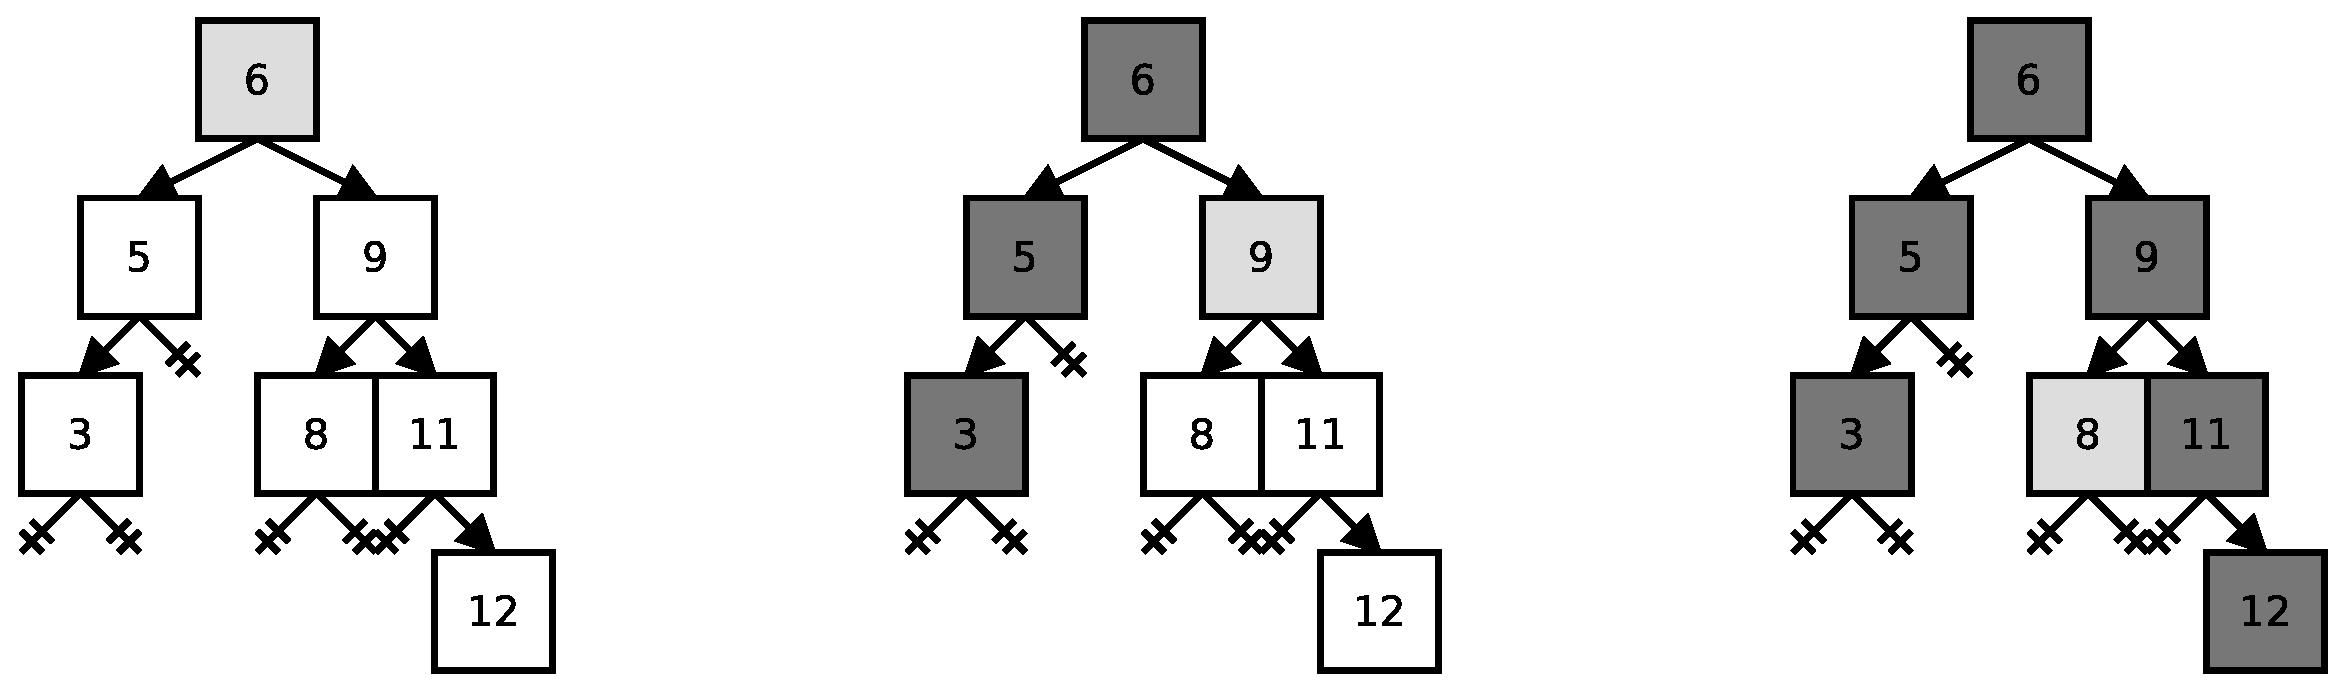
\includegraphics[width=\textwidth]{gfx/tree-find}
  \caption{Finding elements in a tree. Every time we check an element
    to find the one we are looking for, we discard half of the
    remaining elements. In this example, finding the element
    containing number 8 requires only three comparisons.}
  \label{fig:fhsdhshgfhjsdg}
\end{figure}

\subsection{Conclusion}
\label{sec:conclusion}

Tress are a useful data structure to keep data sorted with minimal
effort, in a simple and efficient manner. Having the data sorted at
all times makes it easier to find what we are looking for. On the
other hand, trees are more complex data structures than lists
so if the data does not need to be sorted, a list is preferrable. 

\begin{table}[hbtp]
  \centering
  \begin{tabular}{|l|c|c|}
    \hline
    & List & Tree \\
    \hline
    Min. pointers / element & 1 & 2 \\
    Auto-Sorted & No & Yes \\
    Time needed & Linear & Logarithmic \\
    \hline
  \end{tabular}
  \caption{Lists vs. Trees: lists are not sorted 
    while trees are always sorted; time to find an item in a list grows
    linearly with the list's size, while the time required to find an
    element in a tree grows logarithmicly with the size of the tree. 
    (Lists may be sorted, but it needs special insertion methods or
    frequent re-sorting). 
  }
  \label{tab:treelist}
\end{table}


%%% Local Variables:
%%% mode: latex
%%% TeX-master: "main"
%%% End:
